\documentclass{standalone}
%\usepackage{tikz}
%\usetikzlibrary{arrows.meta}
\usepackage{pgfplots}
\pgfplotsset{compat = newest}
%\tikzset{>=Latex}
\usepackage{tikz}
\usetikzlibrary{arrows.meta}
\tikzset{label/.style = {inner sep=1pt, fill=white}}
%\tikzset{nd/.style={circle, inner sep=0pt}}
\tikzset{nd/.style={inner sep=1pt}}
\tikzset{>=Latex}
\tikzset{arc/.style = {->, semithick, >=Latex}}
\begin{document}
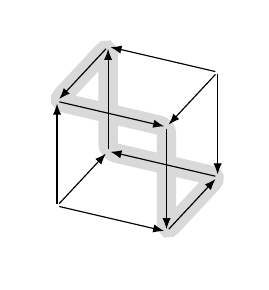
\begin{tikzpicture}[scale=.7]
\begin{axis}[
    axis line style = {opacity=0},
    %xlabel={$P_1$},
    %ylabel={$P_2$},
    %zlabel={$P_3$},
    xmin=-0.1, xmax=1.1,
    ymin=-0.1, ymax=1.1,
    zmin=-0.1, zmax=1.1,
    axis equal image,
    %ticks =none,
    %xtick = 0,
    xticklabels = {},
    %ytick = {0,1},
    yticklabels = {},
    %ztick = {0,1},
    zticklabels = {},
    xtick style = {draw=none},
    ytick style = {draw=none},
    ztick style = {draw=none},
]

    \draw [rounded corners, color = gray!30, line width = 10pt] (1,0,1) to (0,0,1) to (0,1,1) to (0,1,0) to (1,1,0) to (1,0,0) -- cycle;

    %\node (H1) at (-2,0) {$H$:};
    %\node (T1) at (-0.8,1) {$T$:};
    
    \node[nd] (hhh) at (0,0,0) {};
    \node[nd] (thh) at (1,0,0) {};
    \node[nd] (hht) at (0,0,1) {};
    \node[nd] (tht) at (1,0,1) {};
    
    \node[nd] (hth) at (0,1,0) {};
    \node[nd] (tth) at (1,1,0) {};
    \node[nd] (htt) at (0,1,1) {};
    \node[nd] (ttt) at (1,1,1) {};
    
    %\node (o) at (-2.5,-1) {$H$};
    %\node (z) at (-1,-0.2) {$T$};
    %\node (x) at (-0.9,-1) {$T$};
    %\node (y) at (-2.5,0.5) {$T$};
    %\draw (o) -- node[above] {$P_2$} (z);
    %\draw (o) -- node[below] {$P_1$} (x);
    %\draw (o) -- node[left] {$P_3$} (y);
    
    \draw[arc] (hhh) to (hht);
    \draw[arc] (hhh) to (hth);
    \draw[arc] (hhh) to (thh);
    \draw[arc] (ttt) to (htt);
    \draw[arc] (ttt) to (tth);
    \draw[arc] (ttt) to (tht);
    \draw[arc] (htt) to (hht);
    \draw[arc] (hht) to (tht);
    \draw[arc] (hth) to (htt);
    \draw[arc] (tth) to (hth);
    \draw[arc] (thh) to (tth);
    \draw[arc] (tht) to (thh);
\end{axis}
 \end{tikzpicture}
\end{document}